\begin{figure*}
\centering
\begin{subfigure}[b]{0.48\textwidth}
    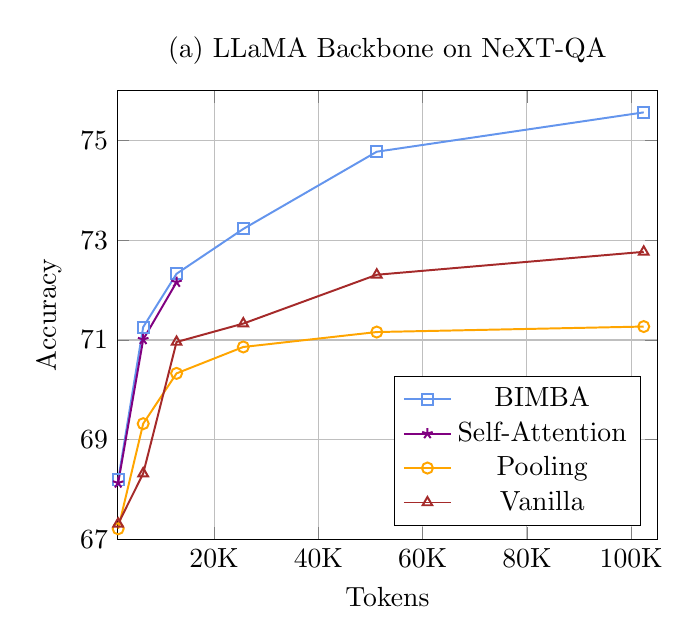
\begin{tikzpicture}
    \begin{axis}[
        % width=12cm, height=8cm,
        xlabel={Tokens},
        ylabel={Accuracy},
        title={(a) LLaMA Backbone on NeXT-QA},
        xmin=1500, xmax=105000,
        ymin=67, ymax=76,
        %xtick={1600, 6400, 12800, 25600, 51200, 102400},
        % xticklabels={1600, 6400, 12800, 25600, 51200, 102400},
        xtick={20000,40000,60000,80000,100000},
        xticklabels={20K, 40K, 60K, 80K, 100K},
        ytick={67, 69, 71, 73, 75, 77},
        legend pos=south east,
        grid=both,
        scaled ticks = false,
        scaled x ticks = false,
        % xmode=log,
        % log basis x=1
    ]
    % BIMBA Data
    \addplot[line width=.25mm, color=CornflowerBlue, mark=square, mark size=2pt]
    coordinates {
    (1600, 68.19) (6400, 71.26) (12800, 72.33) (25600, 73.23) (51200, 74.78) (102400, 75.57)
    };
    \addlegendentry{BIMBA}
    
    % Self-Attention Data
    \addplot[line width=.25mm, color=Purple, mark=star, mark size=2pt]
        coordinates {
        (1600, 68.13) (6400, 71.01) (12800, 72.16) 
    };
    \addlegendentry{Self-Attention}
    
    % Pooling Data
    \addplot[line width=.25mm, color=Orange, mark=o, mark size=2pt]
    coordinates {
    (1600, 67.21) (6400, 69.32) (12800, 70.33) (25600, 70.86) (51200, 71.16) (102400, 71.27)
    };
    \addlegendentry{Pooling}
    \addplot[line width=.25mm, color=Brown, mark=triangle, mark size=2pt]
    coordinates {
    (1600, 67.31) (6400, 68.32) (12800, 70.96) (25600, 71.33) (51200, 72.31) (102400, 72.77)
    };
    \addlegendentry{Vanilla}

    \end{axis}
    \end{tikzpicture}
% \caption{Figure 1}
\end{subfigure}
\hfill
\begin{subfigure}[b]{0.48\textwidth}
    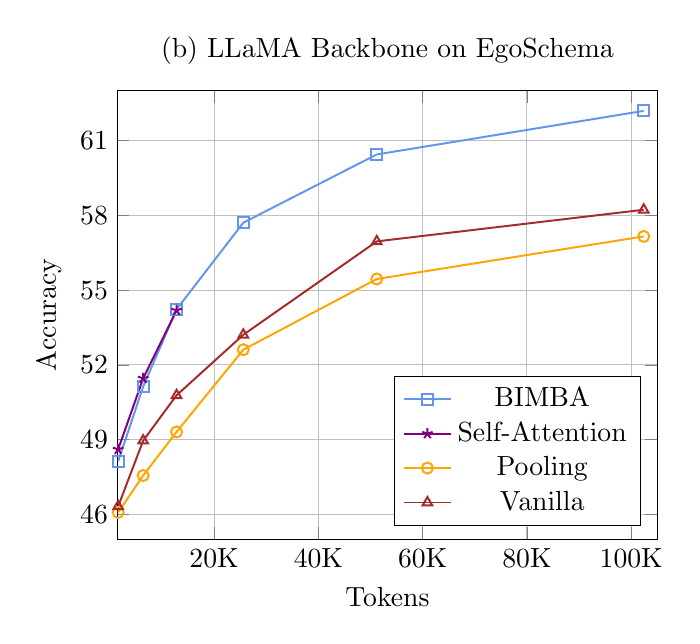
\begin{tikzpicture}
    \begin{axis}[
        % width=12cm, height=8cm,
        xlabel={Tokens},
        ylabel={Accuracy},
        title={(b) LLaMA Backbone on EgoSchema},
        xmin=1500, xmax=105000,
        ymin=45, ymax=63,
        %xtick={1600, 6400, 12800, 25600, 51200, 102400},
        % xticklabels={1600, 6400, 12800, 25600, 51200, 102400},
        xtick={20000,40000,60000,80000,100000},
        xticklabels={20K, 40K, 60K, 80K, 100K},
        ytick={46, 49, 52, 55, 58, 61},
        legend pos=south east,
        grid=both,
        scaled ticks = false,
        scaled x ticks = false,
        % xmode=log,
        % log basis x=1
    ]
    % BIMBA Data
    \addplot[line width=.25mm, color=CornflowerBlue, mark=square, mark size=2pt]
    coordinates {
    (1600, 48.13) (6400, 51.13) (12800, 54.23) (25600, 57.71) (51200, 60.45) (102400, 62.20)
    };
    \addlegendentry{BIMBA}
    
    % Self-Attention Data
    \addplot[line width=.25mm, color=Purple, mark=star, mark size=2pt]
        coordinates {
        (1600, 48.61) (6400, 51.46) (12800, 54.19)
    };
    \addlegendentry{Self-Attention}

    % Pooling Data
    \addplot[line width=.25mm, color=Orange, mark=o, mark size=2pt]
    coordinates {
    (1600, 46.08) (6400, 47.56) (12800, 49.31) (25600, 52.61) (51200, 55.45) (102400, 57.16)
    };
    \addlegendentry{Pooling}

    \addplot[line width=.25mm, color=Brown, mark=triangle, mark size=2pt]
    coordinates {
    (1600, 46.32) (6400, 48.96) (12800, 50.78) (25600, 53.21) (51200, 56.96) (102400, 58.23)
    };
    \addlegendentry{Vanilla}
    
    \end{axis}
    \end{tikzpicture}
    % \caption{Figure 2}
\end{subfigure}
\caption{Performance Using LLaMA-3.2 Backbone}
\label{fig:performance llama}
\end{figure*}